%!TEX root = ../Thesis.tex
\section{Dokumentation der Software}
\fancyhead[R]{Dokumentation der Software}
\label{instal}

\subsection{Dokumentation der Paketstruktur (Sertan Cetin)}
%%%%%%%%%%%
%Sertan
%%%%%%%%%%%
 
\subsection{Dokumentation der Activities}
%%%%%%%%%%%
%Alle
%%%%%%%%%%%

\subsubsection{Main Activity}

%Fabia
\textbf{Layouts (Fabia Schmid)}\\
Das Layout der Overview Activity orientiert sich an dem vorher erstellten Mockup und besteht aus drei Grundkomponenten. Es gibt am oberen Bildschirmrand eine Leiste zum Erstellen von Notes, Events und ToDos, sowie ein Button zum Suchen. Unter dieser leiste befindet sich ein Container, welcher die verschiedenen Fragments der vorhandenen Notes, Events und ToDos beinhaltet. Am unteren Bildschirmrand befindet sich noch eine Leiste mit vier Buttons zum Filtern der  Fragments.

\begin{figure}[H]
\centering
\begin{minipage}[t]{1\textwidth} % Breite, z.B. 1\textwidth		
\caption{Overview Activity} % Überschrift
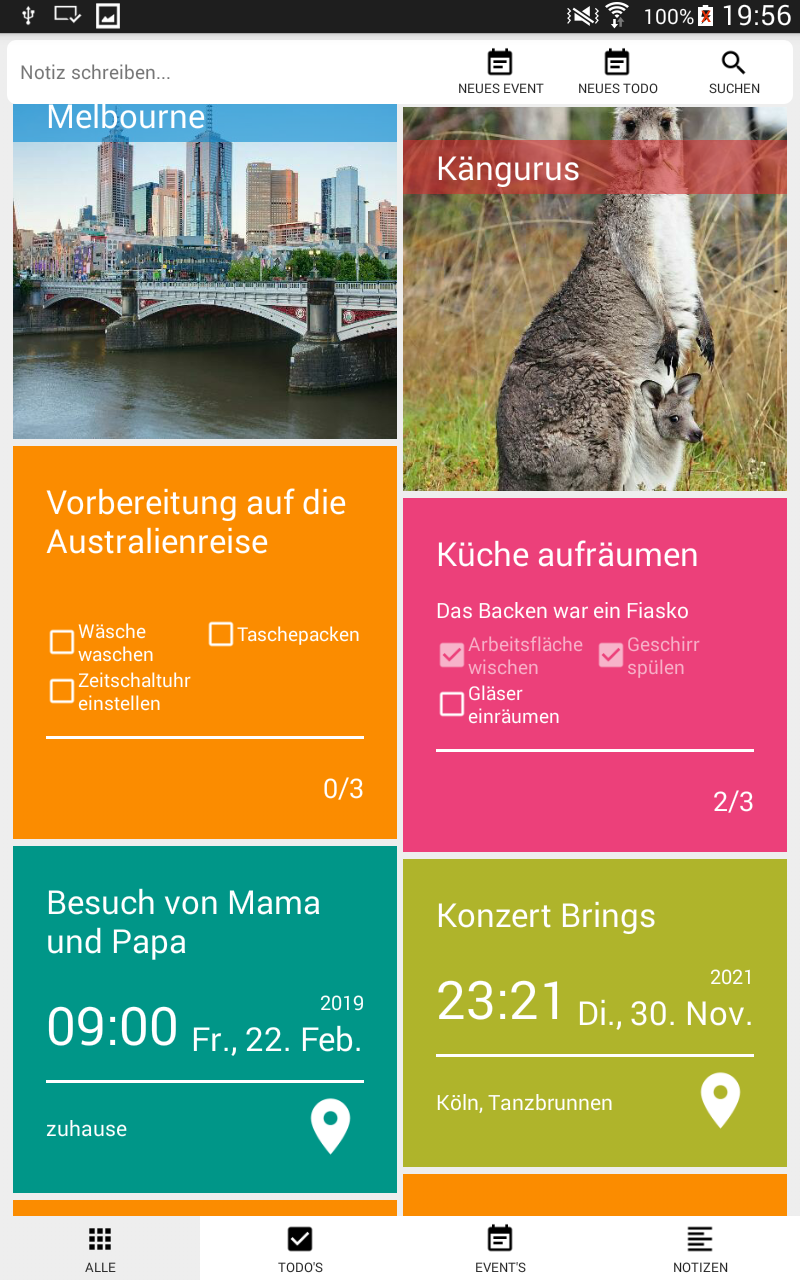
\includegraphics[width=1\textwidth]{img/Overview}\\ % Pfad
\source{Screenshot aus der Benutzeroberfläche} % Quelle
\end{minipage}
\end{figure}

Die Activity Overview zeigt normal 2 Spalten mit Fragments, wenn jedoch das Tablet gedreht wird zeigt die Landscape-Ansicht drei Spalten mit Fragments, um den Bildschirm optimal zu nutzen.

\begin{figure}[H]
\centering
\begin{minipage}[t]{1\textwidth} % Breite, z.B. 1\textwidth		
\caption{Landscape Ansicht - Overview Activity} % Überschrift
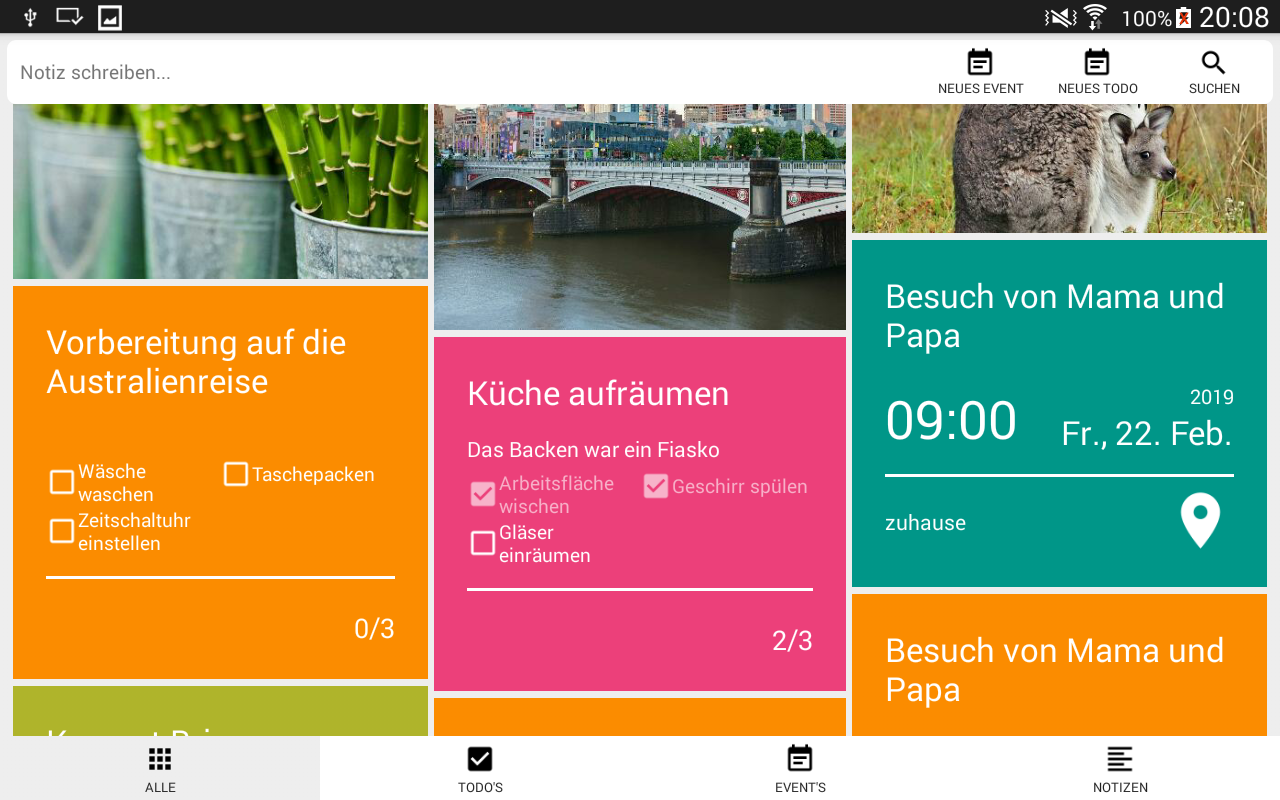
\includegraphics[width=1\textwidth]{img/Landscape}\\ % Pfad
\source{Screenshot aus der Benutzeroberfläche} % Quelle
\end{minipage}
\end{figure}

Die drei verschiedenen Arten von Fragments sind Notes, ToDo und Event.

Bei einer Note wird die Überschrift und ein Textauszug angezeigt. Wenn jedoch ein Bild in der Notiz vorhanden ist wird dieses mit der Überschrift in der Overview Activity angezeigt.

\begin{figure}[H]
\centering
\begin{minipage}[t]{1\textwidth} % Breite, z.B. 1\textwidth		
\caption{Note Fragments} % Überschrift
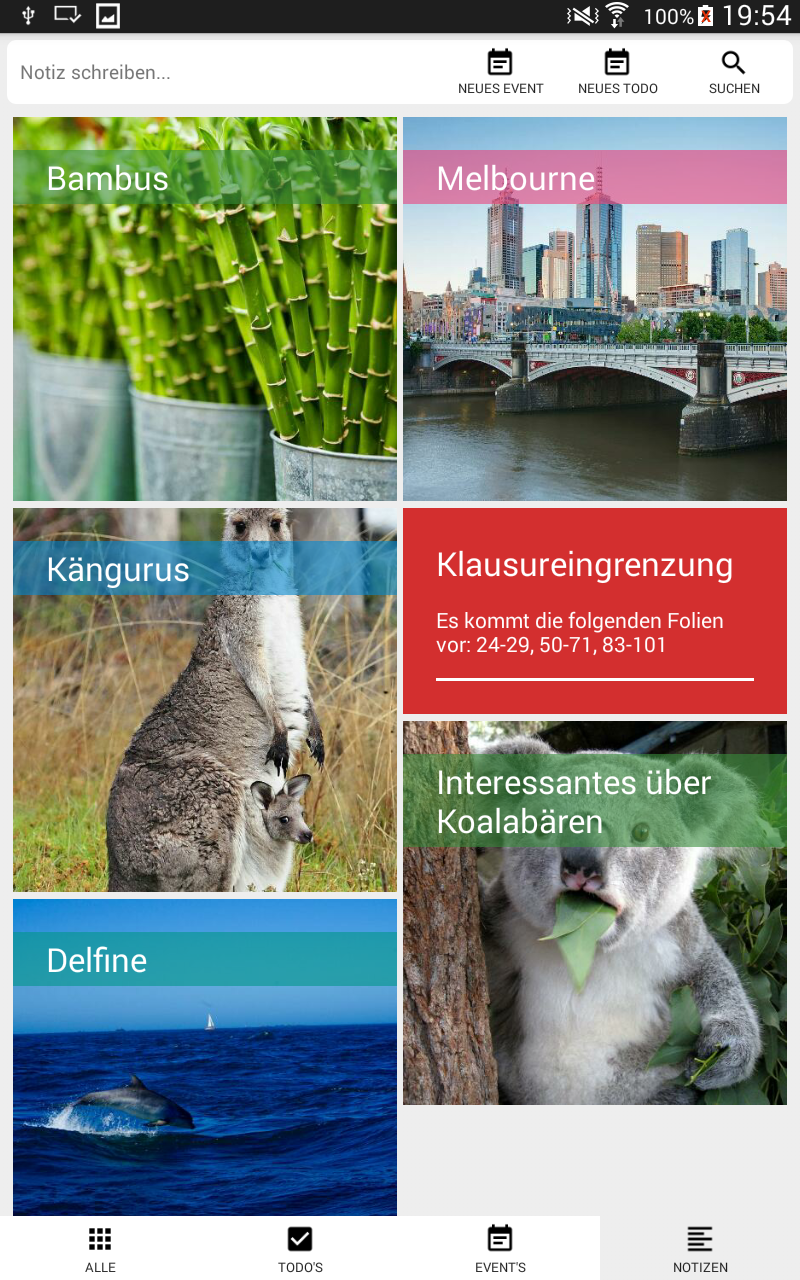
\includegraphics[width=1\textwidth]{img/FragmentN}\\ % Pfad
\source{Screenshot aus der Benutzeroberfläche} % Quelle
\end{minipage}
\end{figure}

Die Fragments für die ToDos, zeugen auch den Titel an und die einzelnen Aufgaben mit Kästchen, die mit einem Hacken gefüllt sind, wenn sie erledigt sind. Zusätzlich wird Angezeigt, wie viele Aufgaben schon erfüllt wurden.

\begin{figure}[H]
\centering
\begin{minipage}[t]{1\textwidth} % Breite, z.B. 1\textwidth		
\caption{Todo Fragments} % Überschrift
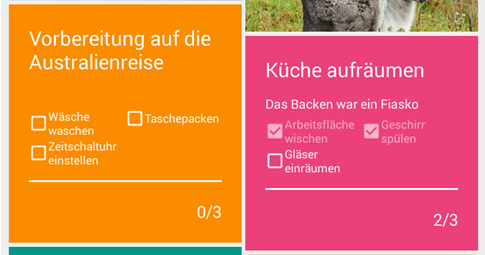
\includegraphics[width=1\textwidth]{img/FragmentT}\\ % Pfad
\source{Screenshot aus der Benutzeroberfläche} % Quelle
\end{minipage}
\end{figure}

Die Event Fragmentes bestehen aus der Überschrift, dem Datum und der Uhrzeit, sowie aus einem Ort, der angegeben werden kann.

\begin{figure}[H]
\centering
\begin{minipage}[t]{1\textwidth} % Breite, z.B. 1\textwidth		
\caption{Event Fragments} % Überschrift
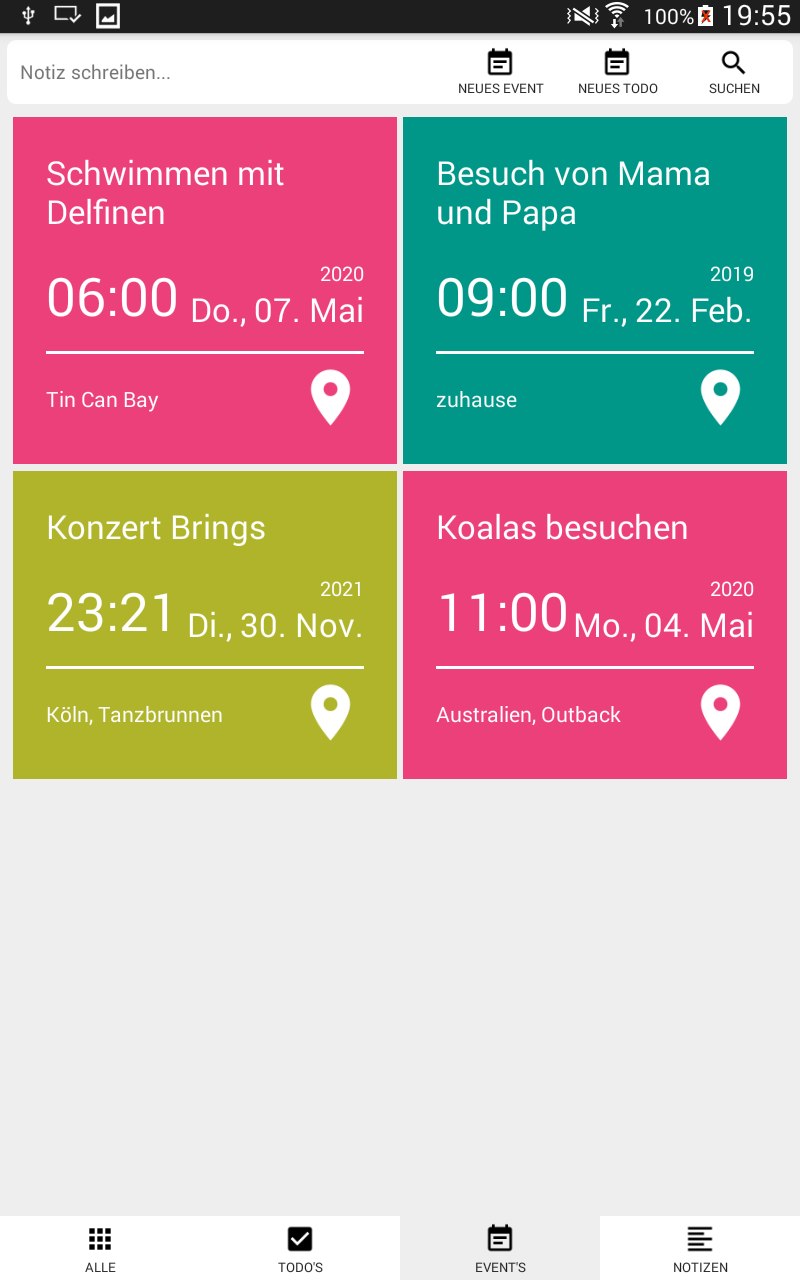
\includegraphics[width=1\textwidth]{img/FragmentE}\\ % Pfad
\source{Screenshot aus der Benutzeroberfläche} % Quelle
\end{minipage}
\end{figure}

In der Overview Activity kann zusätzlich gesucht und gelöscht werden. Wenn man einen langen Click auf ein Fragment macht, wird die obere Leiste verändert und man bekommt einen Button zum Löschen. Zusätzlich kann in dieser Ansicht nun auf die verschiedenen Fragments geklickt werden, um diese zu markieren und mehrere gleichzeitig zu löschen. Diese Ansicht kann durch den Zurück-Pfeil verlassen werden.

\begin{figure}[H]
\centering
\begin{minipage}[t]{1\textwidth} % Breite, z.B. 1\textwidth		
\caption{Overview Activity - Löschen} % Überschrift
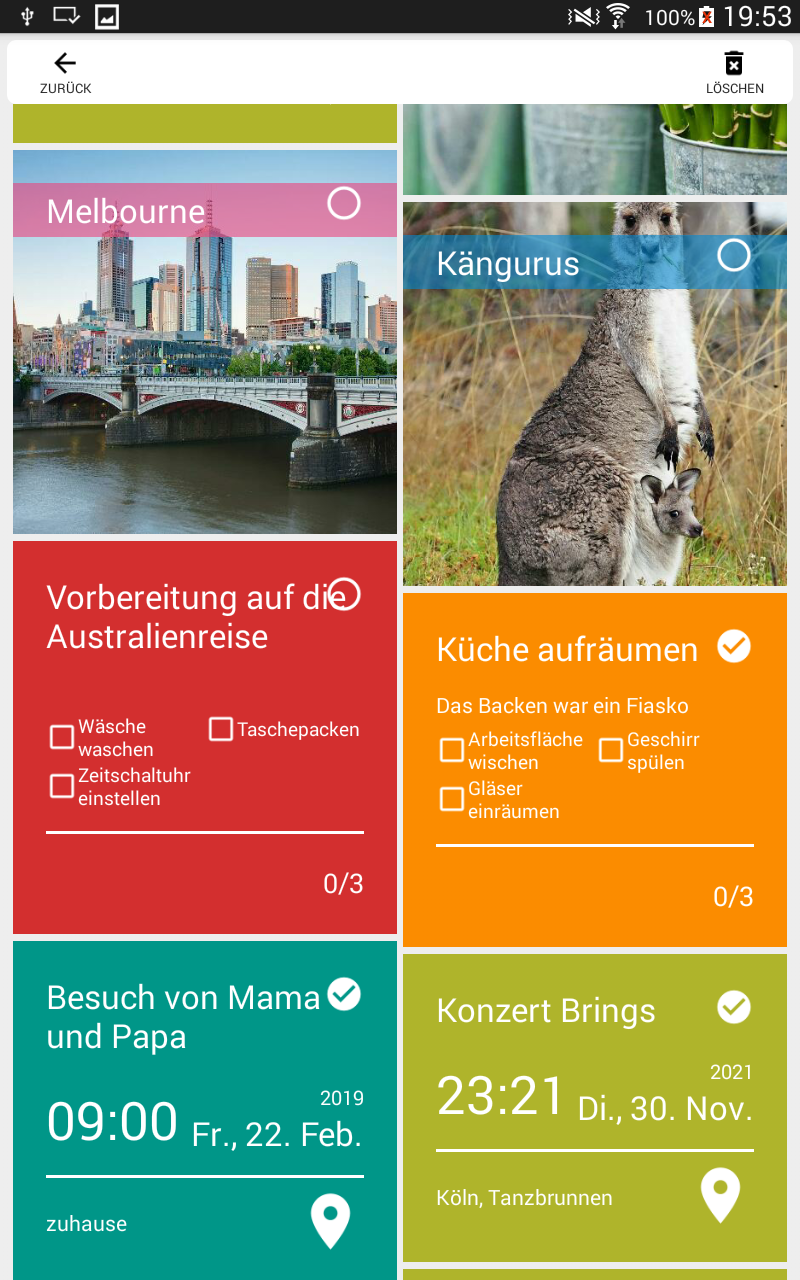
\includegraphics[width=1\textwidth]{img/Loeschen}\\ % Pfad
\source{Screenshot aus der Benutzeroberfläche} % Quelle
\end{minipage}
\end{figure}

Auch bei der Suchfunktion wird die obere Leiste angepasst. Dabei kann nun ein beliebiges Wort eingegeben werden, welches dann in den verschiedenen Einträgen gesucht wird. Die gefundenen Einträge werden daraufhin angezeigt. Um die Suche zu beenden kann der Zurück-Pfeil verwendet werden.

\begin{figure}[H]
\centering
\begin{minipage}[t]{1\textwidth} % Breite, z.B. 1\textwidth		
\caption{Overview Activity - Suchen} % Überschrift
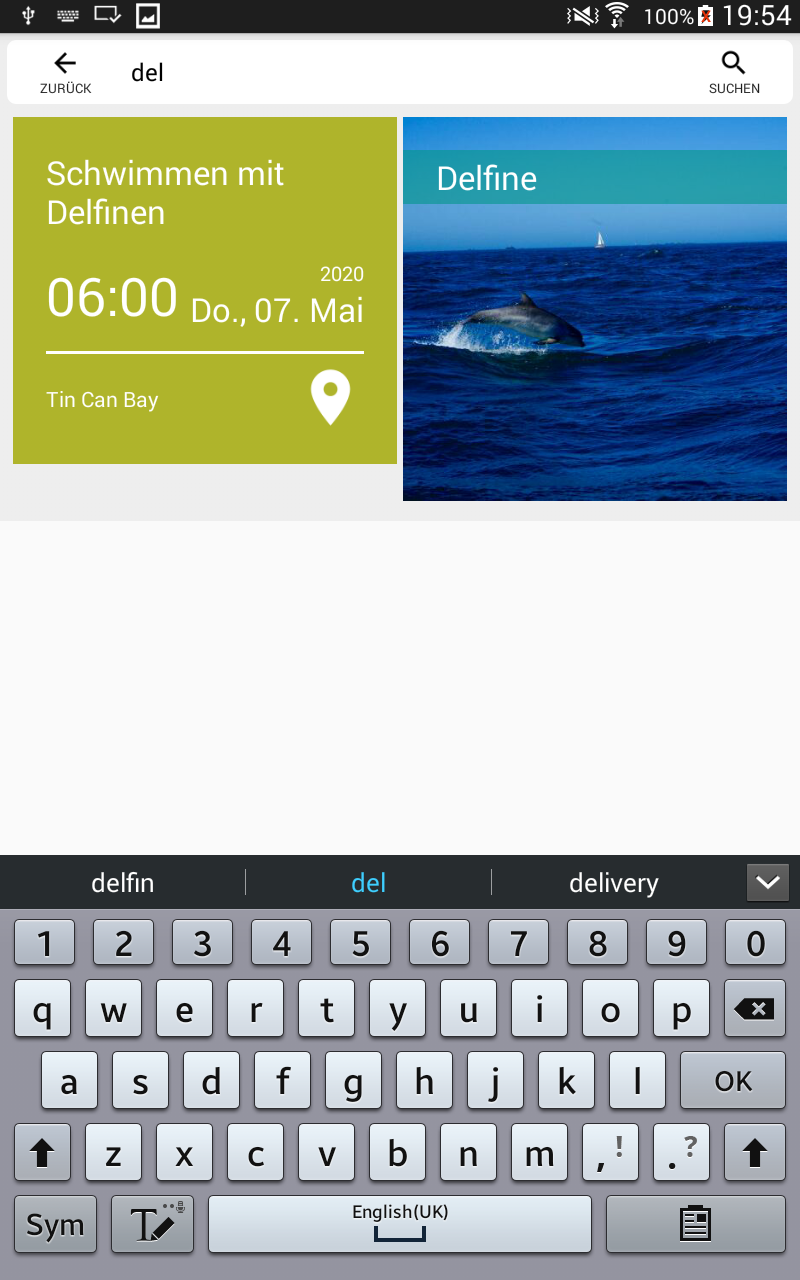
\includegraphics[width=1\textwidth]{img/Suchen}\\ % Pfad
\source{Screenshot aus der Benutzeroberfläche} % Quelle
\end{minipage}
\end{figure}

\subsection{Dokumentation der Navigation zwischen Activities (Yannick Rüttgers)}
%%%%%%%%%%%
%Yannick
%%%%%%%%%%%

Hier den Text einfach hin kopieren.

\subsection{Dokumentation der Activity-übergreifenden, persistenten Datenhaltung (Jan Beilfuß)}
%%%%%%%%%%%
%Jan
%%%%%%%%%%%

Hier den Text einfach hin kopieren.

\newpage
\subsection{Dokumentation der Activity-übergreifenden Klassen (Ruthild Gilles)}
%%%%%%%%%%%
%Ruthild
%%%%%%%%%%%

Zu den Activity-übergreifenden Klassen gehören abgesehen von den Query-Klassen für die persistente Datenhaltung auch die Service-Klassen und die Models-Klassen. Die Models-Klassen enthalten die TEN-Klasse und die einzelnen Todo-, Event- und Note-Klassen. Hier sind auch weitere Util-Klassen untergeordnet. In den Service-Klassen sind Methoden enthalten, die die Schnittstelle zwischen Datenbank und Activities darstellen. Im Folgendem wird genauer auf die einzelnen Klassen eingegangen.

\subsubsection{Models-Klassen}

\subsubsection{Service-Klassen}

Damit die Activities die Daten der TEN-Objekte auf der dokumentenbasierten Datenbank speichern können, wurden Service Klassen implementiert. Hierzu gehörten hauptsächlich Klassen zum Erzeugen neuer TEN-Objekte (Create), zum Erhalten bereits gespeicherter TEN-Objekte von der Datenbank (Read), zum Speichern veränderter TEN-Objekte (Update) und zum Löschen von TEN-Objekten von der Datenbank (Delete). Diese sogenannte CRUD-Operationen wurden in den entsprechenden Klassen teilweise für alle drei verschiedenen Objekttypen einzeln eingefügt, teilweise aber auch für TEN-Objekte im Allgemeinen. Dank Polymorphie können die jeweils einzelnen Objekttypen ebenfalls an die entsprechenden Methoden übergeben werden.

Diese Struktur wurde während der Planungsphase vom Datenteam überlegt und während der Implementierung angepasst. Wie auch schon in der Planungsphase definiert enthält die Create-Klasse Methoden, die ein neues leeres Todo, Event oder Note zurückgeben. Diese Methode ruft den Konstruktor der jeweiligen TEN-Klasse auf. Eine Interaktion mit der Datenbank ist hier noch nicht nötig.

Die Read-Klasse hingegen muss auf die Datenbank zugreifen, um entweder alle TEN-Objekte an die Main-Activity in einem ListArray zu übergeben oder aber ein spezielles Todo, Event oder Note, welches von den einzelnen Todo-, Event- oder Note-Activities aufgerufen werden kann. Damit das gewünschte TEN-Objekt in der Datenbank gefunden werden kann, benötigen die Read-Methoden die ID des gewünschten Objektes. Dieses wird als String beim Aufruf der jeweiligen Methode übergeben.

Die Update-Klasse dient zum Speichern von Änderungen an Todo-, Event- und Note-Objekten. Dazu überprüft die Methode, der ein TEN-Objekt übergeben wurde, ob dieses bereits auf der Datenbank existiert. Ist dies der Fall, wird eine Methode zum Ausführen des Update-Befehls auf der Datenbank aufgerufen. Ist dies nicht der Fall, wird eine Methode zum Ausführen des Insert-Befehls auf der Datenbank aufgerufen. Da die Todo-, Event- und Note-Klassen von der TEN-Klasse erben, kann hier Polymorphie angewandt werden. Es ist nur eine Methode zum Speichern notwendig.

Für das Löschen von TEN-Objekten sind in der Delete-Klasse zwei Methode vorhanden. Die eine löscht nur ein übergebenes TEN-Objekt aus der Datenbank, indem es eine entsprechende Methode aus einer der Repository-Klassen aufruft und dieser die ID des TEN-Objektes übergibt. Sollen jedoch mehrere TEN-Objekte auf einmal gelöscht werden, kann der zweiten Methode eine Array List, die mehrere zu löschende Objekte enthält, übergeben werden. Dabei müssen die Objekte nicht alle von dem gleichen Datentyp sein, sondern können Todo-, Event- und Note-Objekte enthalten. Die Methode iteriert durch die übergebene Array List und ruft für jeden Eintrag die Methode zum Löschen eines Objektes auf.


